\documentclass[12pt]{article}
\usepackage{graphicx}
\usepackage{amsmath}
\usepackage{fullpage}
\usepackage{amssymb}
\usepackage{amsfonts}
\usepackage{latexsym}
%\usepackage{pstricks}
\usepackage{tikz,pgflibraryplotmarks}
\usepackage{algorithm}
\usepackage{algpseudocode}
\usepackage{hyperref}
\usepackage[nottoc,numbib]{tocbibind} 
\usepackage{todonotes}


\newcommand{\bfA}	{{\bf{A}}}
\newcommand{\bfB}	{{\bf{B}}}
\newcommand{\bfC}	{{\bf{C}}}
\newcommand{\bfD}	{{\bf{D}}}
\newcommand{\bfE}	{{\bf{E}}}
\newcommand{\bfF}	{{\bf{F}}}
\newcommand{\bfG}	{{\bf{G}}}
\newcommand{\bfH}	{{\bf{H}}}
\newcommand{\bfI}	{{\bf{I}}}
\newcommand{\bfJ}	{{\bf{J}}}
\newcommand{\bfK}	{{\bf{K}}}
\newcommand{\bfL}	{{\bf{L}}}
\newcommand{\bfM}	{{\bf{M}}}
\newcommand{\bfN}	{{\bf{N}}}
\newcommand{\bfO}	{{\bf{O}}}
\newcommand{\bfP}	{{\bf{P}}}
\newcommand{\bfQ}	{{\bf{Q}}}
\newcommand{\bfR}	{{\bf{R}}}
\newcommand{\bfS}	{{\bf{S}}}
\newcommand{\bfT}	{{\bf{T}}}
\newcommand{\bfU}	{{\bf{U}}}
\newcommand{\bfV}	{{\bf{V}}}
\newcommand{\bfW}	{{\bf{W}}}
\newcommand{\bfX}	{{\bf{X}}}
\newcommand{\bfY}	{{\bf{Y}}}
\newcommand{\bfZ}	{{\bf{Z}}}

\newcommand{\bfa}	{{\bf{a}}}
\newcommand{\bfb}	{{\bf{b}}}
\newcommand{\bfc}	{{\bf{c}}}
\newcommand{\bfd}	{{\bf{d}}}
\newcommand{\bfe}	{{\bf{e}}}
\newcommand{\bff}	{{\bf{f}}}
\newcommand{\bfg}	{{\bf{g}}}
\newcommand{\bfh}	{{\bf{h}}}
\newcommand{\bfi}	{{\bf{i}}}
\newcommand{\bfj}	{{\bf{j}}}
\newcommand{\bfk}	{{\bf{k}}}
\newcommand{\bfl}	{{\bf{l}}}
\newcommand{\bfm}	{{\bf{m}}}
\newcommand{\bfn}	{{\bf{n}}}
\newcommand{\bfo}	{{\bf{o}}}
\newcommand{\bfp}	{{\bf{p}}}
\newcommand{\bfq}	{{\bf{q}}}
\newcommand{\bfr}	{{\bf{r}}}
\newcommand{\bfs}	{{\bf{s}}}
\newcommand{\bft}	{{\bf{t}}}
\newcommand{\bfu}	{{\bf{u}}}
\newcommand{\bfv}	{{\bf{v}}}
\newcommand{\bfw}	{{\bf{w}}}
\newcommand{\bfx}	{{\bf{x}}}
\newcommand{\bfy}	{{\bf{y}}}
\newcommand{\bfz}	{{\bf{z}}}

\newcommand{\A}		{\vec{A}}
\newcommand{\B}		{\vec{B}}
\newcommand{\C}		{\vec{C}}
\newcommand{\D}		{\vec{D}}
\newcommand{\E}		{\vec{E}}
\newcommand{\F}		{\vec{F}}
\newcommand{\G}		{\vec{G}}
\renewcommand{\H}	{\vec{H}}
\newcommand{\I}		{\vec{I}}
\newcommand{\J}		{\vec{J}}
\newcommand{\K}		{\vec{K}}
\renewcommand{\L}	{\vec{L}}
\newcommand{\M}		{\vec{M}}
\newcommand{\N}		{\vec{N}}
\renewcommand{\O}	{\vec{O}}
\renewcommand{\P}	{\vec{P}}
\newcommand{\Q}		{\vec{Q}}
\newcommand{\R}		{\vec{R}}
\renewcommand{\S}	{\vec{S}}
\newcommand{\T}		{\vec{T}}
\newcommand{\U}		{\vec{U}}
\newcommand{\V}		{\vec{V}}
\newcommand{\W}		{\vec{W}}
\newcommand{\X}		{\vec{X}}
\newcommand{\Y}		{\vec{Y}}
\newcommand{\Z}		{\vec{Z}}

\newcommand{\hf}        {{\frac 12}}
\newcommand{\bfepsilon} {{\boldsymbol \epsilon}}
\newcommand{\bfsigma}   {{\boldsymbol \sigma}}
\newcommand{\bfSigma}   {{\boldsymbol \Sigma}}
\newcommand{\bfOmega}   {{\boldsymbol \Omega}}
\newcommand{\bfGamma}   {{\boldsymbol \Gamma}}
\newcommand{\bfgamma}   {{\boldsymbol \gamma}}
\newcommand{\bfPhi}     {{\boldsymbol \Phi}}
\newcommand{\bflambda}  {{\boldsymbol \lambda}}
\newcommand{\bfmu}      {{\boldsymbol \mu}}
\newcommand{\bfeta}     {{\boldsymbol \eta}}

\newcommand{\bfmhat}    {{\widehat{\bfm}}}
\newcommand{\bfdhat}    {{\widehat{\bfd}}}
\newcommand{\LtL}       { \bfL^{\top}\bfL}

\newcommand {\vu}  	 {{\vec {\bf  u}} }   % continuous flow field
\newcommand {\vuref} {\vu_{\text{ref}}}  % continuous reference flow field
\newcommand {\vq}  	 { {\vec {\bf  q}} }
\newcommand {\ve}    { {\vec {\bf  e}} }
\newcommand {\vh}    { {\vec {\bf  h}} }
\newcommand {\vx}    {\vec {\bf x}}     
\newcommand {\bx}    {{\bf{x}}}     
   
\renewcommand {\bflambda}  { {\boldsymbol{\lambda}}}     
\newcommand {\blambda}	 { {\boldsymbol \lambda} }
\newcommand {\bmu}    	 { {\boldsymbol \mu} }
\newcommand {\zero}   	 { {\bf 0} }
\newcommand {\bnabla}	 { { \boldsymbol \nabla} }
\newcommand {\btheta}	 { { \boldsymbol \theta} }
\newcommand {\balpha}	 { { \boldsymbol \alpha} }
\newcommand {\bfxi}		 { { \boldsymbol \xi} }
\renewcommand{\hf}		 {\frac12}
\newcommand{\hx}[1]		 {{\ensuremath{h^x_{\scriptscriptstyle #1}}}}
\newcommand{\hy}[1]		 {{\ensuremath{h^y_{\scriptscriptstyle #1}}}}
\newcommand{\hz}[1]		 {{\ensuremath{h^z_{\scriptscriptstyle #1}}}}


\newcommand{\s}		{\vec{s}}
\newcommand{\h}		{\vec{h}}
\newcommand{\n}		{\vec{n}}
\newcommand{\x}		{\vec{x}}
\renewcommand{\u}		{\vec{u}}
\renewcommand{\div}	{\nabla\cdot\,}
\newcommand{\grad}	{\ensuremath {{\bf{ \nabla}}}}
\newcommand{\curl}	{\ensuremath{{\nabla}\times\,}}
\newdimen\iwidth\iwidth=30mm
\newcommand{\rottext}[1]	{\rotatebox{90}{\hbox to 30mm{\hss #1\hss}}}
\newcommand{\rme}			{\rm{e}}
\newcommand{\HRule}			{\rule{\linewidth}{0.25mm}}

\newcommand{\JJ} 	 {\mathcal{J}}    % objective functional
\newcommand{\cD} 	 {\mathcal{D}}    % data misfit
\newcommand{\CR} 	 {\mathcal{R}}    % regularization functional
\newcommand{\CRflow} {\mathcal{R}^{\text{flow}}}    %  flow 
\newcommand{\CRsat}  {\mathcal{R}^{\text{s}}}     %  saturation 
\newcommand{\CF} 	 {\mathcal{F}}    % continuous tomography operator
\newcommand{\sh} 	 {\texttt{s}}     % discretized initial slowness
\newcommand{\DIVh}   {{\textsf{DIV}}}  % discretized divergence 
\newcommand{\CURLh}  {{\textsf{CURL}}} % discrete curl operator
\newcommand{\GRADh}  {{\textsf{GRAD}}} % discrete gradient operator

\renewcommand{\bfmhat}	{\widehat{\bf m}}
\newcommand{\bfwhat}	{\widehat{\bf w}}

\newcommand*\xbar[1]{%
  \hbox{%
    \vbox{%
      \hrule height 0.5pt % The actual bar
      \kern0.5ex%         % Distance between bar and symbol
      \hbox{%
        \kern-0.em%      % Shortening on the left side
        \ensuremath{#1}%
        \kern-0.15em%      % Shortening on the right side
      }%
    }%
  }%
} 
\newcommand{\mbar}	{\xbar{\bf m}}
\newcommand{\wbar}	{\xbar{\bf w}}
\newcommand{\dbar}	{\xbar{\bf d}}
\newcommand{\Fbar}	{\xbar{\bf F}}
\def\kronecker{\raisebox{1pt}{\ensuremath{\:\otimes\:}}} 




\sloppy



\begin{document}

\title{Adaptive A-optimal experimental design for imaging dynamic targets}
\author{J. Fohring and E. Haber }


\maketitle
\begin{abstract}
Efficiently monitoring subsurface flow using geophysical imaging techniques is important to several applications such as aquifer characterization or enhanced oil recovery projects.
One method of increasing monitoring efficiency is to control the number of measurements required for a geophysical survey in an optimal way. To optimally design future geophysical experiments, we use A-optimal design methods while incorporating the flow dynamics.  

 A-optimal design methods minimize the posterior covariance matrix associated with estimating the target subsurface model. We reformulate the MAP estimate for the prior target in order to design for the future target, such that the problem is constrained by the flow dynamics. In this way, the prior experiments collected data and flow dynamics contribute to the design of the next experiment, thus incorporating updated information to the design algorithm. 
 
The method is demonstrated for a two dimensional borehole seismic tomography experiment and a three dimensional seismic survey. An advection model  is applied to describe subsurface flow and  propagate the error covariance matricies forward in time. 
 


\end{abstract}



\section{Introduction} 
\begin{itemize}

\item Monitoring; Many problems in geophysics address the issue of monitoring subsurface flow, such as aquifer characterization, enhanced oil recovery, or saltwater intrusion. In general one would like to image the motion of certain subsurface parameters over a period of time.  One method to do so is to collect measurements dependent on these parameters and invert through a mathematical relationship to recover parameter distributions. When monitoring for these dynamic parameters, the choice of where the data are collected becomes important as resolution is both temporally and spatially dependent. 

\item much has been done in experimental designs for linear and nonlinear problems...A optimal, etc.. appropriate references. As well as for large scale ill posed, refs.  inverting for fluid parameters given geophysical imaging...refs...talk about seismic, and helmoltz and simultaneous sources

\item Determining the design of the data collection experiment requires knowledge of the target parameter distribution. Typically optimal experimental design methods rely on minimizing the posterior error covariance matrix, associated with estimating the target through the inversion of geophysical data. This poses a problem, particularly for static cases, since the point of  the data collection is to image the unknown target. However, if the dynamics governing the motion of the unknown target are known, even to a small degree in accuracy, then it is possible to design the data collection experiment to be conducted in the future as the target moves. In order to design for a future experiment it is necessary to know the initial distribution of target parameters as well as the dynamics. If the initial condition is provided with the dynamics, then either an iterative approach or and all at once approach can be taken to determine date collection designs for a set of time points. 
\item ideally, incorporation of real data in the estimation of historic, but also future experimental designs would lead to the best estimates. Adaptively, chase the target, by recomputing the design after data is collected. 

%\item An all at once method would seek to recover the next design given all previous designs  for a set of time points, and the dynamics.  This method requires an 'all at once' prior covariance matrix.  However, This method puts a great deal of trust into the dynamic model. If for example, the velocity field in which a tracer is advected is known to very low accuracy then the designs and location of the tracer target far into the future would have significant error. Therefore we restrict our future designs to only one time step. 

\item We also consider what happens if we wish to recover/update the parameters governing the fluid flow. How does this change designs for the future time step? 


\item computational limitations: (constrained all at once, no error) no historic info included, (Kalman formulation, error) covariance matrices are large and dense, making factorization/ reduction techniques difficult. geophysical experiments are computationally expensive. (adaptive, constrained)
no covariance matrices to worry about, includes last data set/design, can easily tack on regularization.
\end{itemize}

As a model problem we consider the following dynamical system of simple mass transport, where the
dynamics is given by
\begin{eqnarray}
\label{dynamics}
m_{t} + \div {\vu} m = 0\ \quad m(0,\vx) = m_{0}
\end{eqnarray} 


\section{A-Optimal experimental design } 
The section outlines the optimal experimental design criteria chosen to compute optimal experimental designs for a given model estimation problem, along with the design optimization objective function, and sparsity constraints.

The general approach to compute optimal experimental designs for inverse problems is to minimize the error contained in the covariance matrix of the estimate of the unknown model parameters.  There are many different optimization criteria for minimizing the error covariance matrix, such as A,D, or E- optimality to name a few. Here we choose Bayesian A-optimal experimental design, which minimizes the trace of the error covariance matrix, as it is somewhat easier to deal with numerically.   
\bigskip

Consider the discrete static  ill-posed inverse problem of estimating  model parameters $\bfm \in \mathbb{R}^{N}$ from noisy observation data $\bfd \in \mathbb{R}^{M}$, where the data are given by 
\begin{equation*}
\bfd = \bfF \bfm + {\bfepsilon}.
\end{equation*} 
The imaging forward operator  $\bfF: \mathbb{R}^{N} \rightarrow \mathbb{R}^{M}$ is an $M \times N$ matrix with each row representing an experiment.  The data space $ M = ns \times nr$ is determined by the maximum  number of measurements allowed. 
 
Assuming a Bayesian inversion approach is taken, where the posterior estimate  $\bfmhat$ is conditioned on a known prior distribution $\pi_m = N({\bfmu},\bfSigma)$, and that the error ${\bfepsilon}$ is Gaussian $N(0,\W^{-1})$, the Bayesian posterior estimate is then obtained by minimizing the negative log-likelihood of Bayes rule 
\begin{eqnarray*}
\bfmhat(\bfw) &=& \text{ argmin } \hf\| \bfF \bfm- \bfd\|^2_{ \bfW} + \hf \|\bfm-{\bfmu}\|^2_{\bfSigma^{-1}}\\
 &=& (\bfF^{\top} \bfW \bfF + \bfSigma^{-1})^{-1}(\bfF^{\top} \bfW \bfd + \bfSigma^{-1}{\bfmu}).
\end{eqnarray*}     
 The weighting matrix $\bfW = \text{diag}[\bfw] \text{ with } \bfw = (\omega_1,..,\omega_M)^{\top}$, relates to the data variance as Var($d_{i}$) $=1/\omega_i$. 
 
\bigskip


A-optimal experimental designs  are defined by  minimizing the average variance of the estimate $\bfmhat$, thus minimizing the trace of the posterior covariance matrix of $\bfmhat$ \cite{Atkinson1992}, which leads to the following A-optimal design objective function
  
  \begin{equation}
  \label{AB}
  \phi_{A_B}(\bfw) = \text{tr}[(\bfF^{\top} \bfW \bfF + \bfSigma^{-1})^{-1}].
  \end{equation}


Given $\phi_{A_B}$, an optimal design is  computed by solving a sparsity controlled optimal design optimization problem \cite{Haber2008}. The design weights $\omega_i$ are determined  by minimizing  $\phi(\bfw)$ with an $\l_1$ penalty on  $\bfw$ to promote sparsity,


\begin{eqnarray}
\label{design}
&\widehat{\bfw}& = \text{ arg min } \phi(\bfw) + \beta\|\bfw\|_1\\
\nonumber
 &\text{ s.t.}& 0 \geq \omega_i.
\end{eqnarray}

It is important to note that in this formulation $\bfmhat$ is chosen to be a linear (or affine) function of the data, although  other estimators could be used, such as a Tikhonov estimator. 
Since the idea is to  design experiments at future time steps for linear dynamic problems  where the estimators covariance matrix can be estimated, the simple Bayesian estimator is sufficient.




\section{Designing experiments for dynamic targets}
\label{dynamicDesign}

Let us consider the case of design for a dynamical system.
There are two main cases to be considered. First, if the dynamic is fast compared to the experimental time
then, the design needs to be done prior to $t_{0}$, that is, prior to the evolution of the system.
Such a design has been addressed in \cite{xxx} and it is a direct use of the standard A optimal design
given the dynamics. A second case that needs to be considered is when the dynamics is slow compared
to the experimental time. In this case one has the time to collect the data and process it and then 
change the experimental design given the estimation of the model. 


To begin, consider the discrete  dynamic process and imaging  described  by the following set of linear equations
 \begin{subequations}
\begin{eqnarray}
\label{eq:system}
\bfm _k&=& \bfT\bfm_{k-1} + {\bfeta}_k,\\
\bfd_k &=& \bfF \bfm_k + {\bfepsilon}_k,
\end{eqnarray}  
\end{subequations}
where transport matrix $\bfT: \mathbb{R}^{N} \rightarrow \mathbb{R}^{N}$  is a discretization of the dynamic process and the noise vectors $\eta $ and $\epsilon $ are assumed to be Gaussian normal, $\eta \sim N(\eta_0,\bfSigma_{\eta})$ and ${\bfepsilon} \sim N(\epsilon_0,\bfW^{-1})$, for $k = 1,..,n$ time points.

We further consider two cases. First, if the dynamical system is well understood and modeled in high accuracy
then we can ignore ${\boldsymbol \eta}_k$. In this case, if $\bfm_{0}$ is known then
the whole dynamics is determined and therefore,  this case 
 leads to the estimation of the initial condition $\bfm_{0}$ only.
 A second case is that we assume some noise in the dynamics. In this case we need to take the dynamical
  noise into consideration and need to design and experiment to estimate the model $\bfm_{k}$ given the 
  the previous estimate $\bfm_{k-1}$ and the its variance.
  We now discuss these cases.
 
 

%As mentioned above, there are several ways to look at this problem when considering how to estimate and design for $\bfm_k$. We could argue that the noise in the dynamics is insignificant, set $\eta_k = 0,$ and write the system as one equation. This leads to the A-optimal design approach  presented in \cite{Alexanderian2014} and outlined in section \ref{noNoise}, where given a Bayesian estimation for $\bfm_0$, designs are recovered for all subsequent time points.  

%Alternately, we could design for a linear Kalman filter formulation. In Bayesian terms, the dynamics provide all the information for the prior distribution. Estimations for $\bfm_k$ can either be written in an iterative manner, or as an all at once estimation (Kalman smoothing). Designing for the Kalman estimator results in designs for a set of times, without the inclusion of historic data, and where the error associated with the dynamics is propagated in time. This approach is  presented in Section \ref{constrained}. 

%However,  in reality we would like to estimate an optimal design while including information from the previous experiment. To this end we reformulate the estimation of the previous model $\bfm_{k-1}$ by including the constraint $\bfm_k = \bT\bfm_{k-1}$.
%In Section \ref{adaptive} we present this formulation and write the problem as an iterative method that computes an optimal design for a future time point based on the last optimal design. 

\subsection{Design for no noise in dynamics}
\label{noNoise}


Beginning with the simplest case, where $\eta_k = 0$ and assuming $n$ time steps
 we can write the dynamics as block system
of the form
\begin{equation}\label{eq:FlowSystem}
	 \underbrace{
		\left( 
			\begin{array}{rrrrr}
				- \bfI      &           &         &        &        \\
				  \bfT & -\bfI      &         &        &        \\
				           &  \bfT & -\bfI    &        &        \\
				           &           &  \ddots & \ddots &        \\
				           &           &         & \bfT    & -\bfI   \\
			\end{array}
		\right)
	 }_{=: \bfA_{n}}
	 \underbrace{
		\left(
			\begin{array}{r}
				\bfm_1 \\ \bfm_2 \\ \bfm_3 \\ \vdots \\ \bfm_n
			\end{array}
		\right)
	 }_{=: \bfm_{[1:n]}}
	+
	 \underbrace{
		\left(
			\begin{array}{c}
			\bfT \\ 0  \\ 0\\ \vdots \\ 0
			\end{array}
		\right)
	 }_{=: -\bfB_{n}}
	\bfm_0
	= 
	{\zero}.
\end{equation}
Thus, the set of time dependent models can then be written as the solution to the simple linear system
\begin{equation}
\bfm_{[1:n]} = \bfA_{n}^{-1} \bfB_{n} \bfm_0.
\end{equation}
Now, consider that we have done $n-1$ experiments, obtained $n-1$ data vectors 
and that we are seeking to conduct the $n$-th experiment in order
to better evaluate  model, $\bfm_{0}$ at time $n$. The forward problem for all times can be written as
\begin{eqnarray}
\label{foralltimes}
\begin{pmatrix}
\bfd_{1} \\ \bfd_{2} \\ \   \\  \vdots \\ \bfd_{n}
\end{pmatrix} = 
\begin{pmatrix}
\bfF_{1}      &           &         &        &        \\
     & \bfF_{2}      &         &        &        \\
           &  &      &        &        \\
	  &           &   & \ddots &        \\
	 &           &         &     & \bfF_{n}   \\
\end{pmatrix}
\begin{pmatrix}
- \bfI      &           &         &        &        \\
 \bfT     & -\bfI      &         &        &        \\
           &  \bfT & -\bfI    &        &        \\
	  &           &  \ddots & \ddots &        \\
	 &           &         & \bfT    & -\bfI   \\
\end{pmatrix}^{-1}
\begin{pmatrix}
\bfT \\ 0  \\ 0\\ \vdots \\ 0
\end{pmatrix}
\bfm_{0}
\end{eqnarray}
In the case that $\bfF_{k} = \bfF$ we can write the forward problem as
\begin{eqnarray}
\label{dalltimes}
\bfd_{[1:n]} = (\bfI_{n} \kronecker \bfF) \bfA_{n}^{-1} \bfB_{n} \bfm_0
\end{eqnarray}
Let $\bfW_{k}$ be the variance of the data at time step $k$ and let
$\bfW_{[1:n]} = {\sf diag}(\bfW_{1},\ldots,\bfW_{n-1}, \bfW_{n})$. Since the experiments at times
$1,\ldots,n-1$ have already been conducted, the variances, $\bfW_{1}, \ldots, \bfW_{n-1}$ are
set. For the $n$-th experiment we can control only the variance of the last time step, $\bfW_{n} = {\sf diag}(\bfw)$.

In Bayesian design, assuming a covariance matrix of the form $\bfSigma_{\bfm_{0}}^{-1} = \bfL^{\top} \bfL$,
the covariance matrix of the estimated model at time $n$ can be directly written as
\begin{eqnarray}
\label{covapost}
\bfSigma_{n} = (\bfB_{n}^{\top}\bfA_{n}^{-\top} (\bfI_{n} \kronecker \bfF)^{\top} \bfW_{[1:n]}(\bfw) (\bfI_{n} \kronecker \bfF) \bfA_{n}^{-1} \bfB_{n} + \bfL^{\top}\bfL)^{-1},
\end{eqnarray}
where we defined $\bfW_{[1:n]}(\bfw) = {\sf diag}(\bfW_{1},\ldots,\bfW_{n-1}, {\sf diag}(\bfw) )$.
 A optimal Bayesian design minimizes the trace of the covariance matrix at time $n$.
 
\bigskip

An interesting observation is to be made here. The A-optimal Bayesian design does not take the data that
was  collected from time $1$ to $n-1$ in order to obtain the design for time $n$. This is a serious flaw of the Bayesian design. Consider that the data indicates that $\bfm_{0}$ is concentrated in a certain region, then, there is no reason
to design an experiment that captures a general $\bfm_{0}$. The important point to be made here is that the data
allows us to re-estimate the model $\bfm_{0}$ beyond our initial knowledge and focus our efforts its evaluation. indeed, given the data $\bfd_{[1:n-1]} =
[\bfd_{1}^{\top},\ldots,\bfd_{n-1}^{\top}]$
the estimated  model at time $n-1$ given the data is
\begin{eqnarray}
\label{modelmean}
 \widehat \bfm_{0}^{(n-1)} &=& 
(\bfB_{n-1}^{\top}\bfA_{n-1}^{-\top} (\bfI_{n-1} \kronecker \bfF)^{\top} \bfW_{[1:n-1]} (\bfI_{n-1} \kronecker \bfF) \bfA_{n-1}^{-1} \bfB_{n-1} + \bfSigma_{\bfm_{0}})^{-1} \\
 \nonumber
&& \bfB_{n-1}^{\top}\bfA_{n-1}^{-\top} (\bfI_{n-1} \kronecker \bfF)^{\top} \bfW_{[1:n-1]} \bfd_{[1:n-1]}
\end{eqnarray}

For time $t_{n}$ we propose to modify the optimization problem, taking the estimated model into consideration
and minimizing
\begin{eqnarray}
\label{minn}
\min_{\bfm_{0}} 
\hf \|(\bfI_{n} \kronecker \bfF) \bfA_{n}^{-1} \bfB_{n} \bfm_{0} - \bfd_{[1:n]} \|_{\bfW_{[1:n]}}^{2}
+ \hf \| \bfL( \bfm_{0} -  \bfm_{0}^{(n-1)}) \|^{2}
\end{eqnarray}








\newpage

Assuming that the imaging technique does not change in time, the  negative log data likelihood is given by
\begin{equation}
\hf \Big\|(\bfI \kronecker \bfF) \bfA(\bfu)^{-1} \bfB(\bfu) \bfm_0- \bar{\bfd} \Big\|^2_{ \xbar{\bfW}} 
\end{equation}
where, $\xbar{\bfW}$ is a block diagonal matrix with diagonal weight matrices $\bfW_1,\bfW_2,...,\bfW_n$ on its main diagonal for  time points $ k = 1,2,...,n$.

Given a prior distribution for $\mbar \sim N(\mbar_{\;0},\bfSigma_{\mbar})$, with $\bfSigma_{\mbar} = \text{blkdiag}(\bfSigma_{\eta_1},..,\bfSigma_{\eta_n})$, the posterior covariance matrix for the Bayes estimate $\bfmhat_0$ is 
\begin{equation}
\label{noNoiseCov}
\bfSigma_{\bfmhat_0} = \Big(((\bfI \kronecker \bfF) \bfA^{-1} \bfB)^{\top}\;
\xbar{\bfW}\;(\bfI \kronecker \bfF) \bfA^{-1} \bfB + \bfSigma_{\mbar}^{-1}\Big)^{-1}
\end{equation}
Thus the Bayesian A-optimal design functional becomes
 \begin{equation}
  \label{AB}
  \phi_{A_B}(\wbar) = \text{tr}\Big[\Big(((\bfI \kronecker \bfF) \bfA^{-1} \bfB)^{\top}\;
\xbar{\bfW}\;(\bfI \kronecker \bfF) \bfA^{-1} \bfB + \bfSigma_{\mbar}^{-1}\Big)^{-1}\Big],
  \end{equation} 
where the designs recovered are for all times points $k=1,...,n$.
 This method was demonstrated in \cite{Alexanderian2014} for and advection diffusion dynamic flow problem.  
 
 Estimating designs in this way requires that we fully accept the accuracy of the dynamics, and that  the prior distribution covariance matrix is known for each experiment to be conducted. Choosing a linear regularization operator $\bfL$ such that $\bfL^{\top}\bfL = \bfSigma_k^{-1}$ is an option to deal with the priors.

%
%
%
\subsection{Noise in the dynamics}
\label{Kalman}
Again we assume that $\bfu$ is known in equations \eqref{eq:system} so that $ \bfT \leftarrow \bfT(\bfu)$ , and that no initial condition is needed since there is error in the estimates of $\bfm$. Denoting $\mbar = [\bfm_1,\bfm_2,...,\bfm_n]^{\top}$ and  a set of data $\bar{\bfd} = [\bfd_1,\bfd_2,...,\bfd_n]^{\top}$ and assuming the initial condition is given by the noise $\eta_0 = \bfm_0$ and $\bfT_0 = \bfI$ we can write 

\begin{equation}\label{eq:FlowSystem}
	 \underbrace{
		\left( 
			\begin{array}{rrrrr}
				 \bfI   &   0   &         &        &        \\
				 -\bfT  & \bfI      &    0     &        &        \\
				           &  -\bfT & \bfI    &   \ddots     &        \\
				           &           &  \ddots & \ddots &      0  \\
				           &           &         & -\bfT    & \bfI   \\
			\end{array}
		\right)
	 }_{=: \bfA}
	 \underbrace{
		\left(
			\begin{array}{r}
				\bfm_1 \\ \bfm_2 \\ \bfm_3 \\ \vdots \\ \bfm_n
			\end{array}
		\right)
	 }_{=: \mbar}	 
		= 
	{\bf 0}.
	\end{equation}
For a time invariant imaging technique, the Bayesian negative log likelihood is given by
\begin{equation}
\label{eq:Ob}
\JJ(\mbar) = \hf \Big((\bfI \kronecker \bfF) \mbar- \bar{\bfd} \Big)^{\top} \xbar{\bfW} \;\; \Big((\bfI \kronecker \bfF)  \mbar-\bar{\bfd} \Big) + \hf \Big(\bfA \mbar\Big)^{\top} \bfSigma_{\mbar}^{-1}\Big(\bfA \mbar \Big)
\end{equation}
where, $\xbar{\bfW}$ is a block diagonal matrix with diagonal weight matrices $\bfW_0,\bfW_1,...,\bfW_n$ on its main diagonal,  and $\bfSigma_{\mbar} = \text{blkdiag}(\bfSigma_{\eta_1},..,\bfSigma_{\eta_n})$.

The posterior covariance matrix obtained after minimizing $\JJ(\mbar)$ for the Bayes estimate $\mbar$ is given by
\begin{equation}
\Big ((\bfI \kronecker \bfF)^{\top}\xbar{\bfW}\;(\bfI \kronecker \bfF)  + \bfA^{\top}\bfSigma_{\mbar}^{-1} \bfA \Big)^{-1}
\end{equation}
Thus, computing an optimal design entails minimizing the trace of the posterior covariance matrix.
Again, 
\begin{equation}
  \label{AB}
  \phi_{A_B}(\wbar) = \text{tr}\Big[\Big ((\bfI \kronecker \bfF)^{\top}\xbar{\bfW}\;(\bfI \kronecker \bfF)  + \bfA^{\top}\bfSigma_{\mbar}^{-1} \bfA \Big)^{-1}],
  \end{equation} 
  This formulation provides another method of designing all of the experiments given the covariance matrices for each time point. The main difference in this formulation than the previous section is that the error is now propagated in time. However, this method still does not incorporate historic designs or collected data, and it requires storing and manipulating large dense covariance matrices.  
  %
  %
  %
\subsection{Adaptive  optimal design}
\label{adaptive}
In this section  we present two reformulations of the model estimation problems such that historic information is included. In this way the future design will depend on information from the previous experiment and the dynamics of the problem. We will consider the formulation with a linear and a non-linear regularization term.

\subsubsection{Linear regularization}
Referring again to equations \eqref{eq:system}, setting $\eta_k = 0$ and assuming $\bfu$ is known, the model objective function is constructed such that the data misfit term for data collected at time $k-1$ and the data misfit term for time $k$ are included,
\begin{equation}
\label{eq:adaptive}
\mathcal{G}(\bfm_{k-1},\bfw_k) = \hf \|\bfF_{k-1}\bfm_{k-1} - \bfd^c_{k-1} \|^2_2 + \hf  \| \bfF \bfT\bfm_{k-1} - \bfd_{k} \|^2_{\bfW_{k}} + \hf \| \bfL\bfm_{k-1} \|^2_2
\end{equation} 
where $\bfF_{k-1} = \bfW_{k-1}\bfF$, and $\bfm_{k} = \bfT \bfm_{k-1}$. The operator $\bfL$ is a smoothing regularization operator. 
One could argue in this instance that the first term including the historic data can be interpreted as a prior such that the regularization term is not necessarily required. In this way, while it appears that this is a frequentist approach, it can still be interpreted as a Bayesian one if both the collected data misfit term and the regularization combine as a prior.

Minimizing equation \eqref{eq:adaptive} with respect to $\bfm_{k-1}$ yields
the posterior covariance matrix 
\begin{equation}
\label{eq:post}
\bfSigma_{k-1}(\bfw_k)= \Big( \bfF_{k-1}^{\top}\bfF_{k-1} +\bfT^{\top} \bfF^{\top} \bfW_k \bfF \bfT + \bfL^{\top}\bfL \Big)^{-1}.
\end{equation}

By formulating the problem in this manner, one can adaptively update optimal designs after each experiment has been carried out.
 
The design functional to then be minimized is given by
%
\begin{equation}
  \label{ABk}
  \phi_k(\bfw_k) = \text{tr}\Big[\Big( \bfF_{k-1}^{\top}\bfF_{k-1} +\bfT^{\top} \bfF^{\top} \bfW_k \bfF \bfT + \bfL^{\top}\bfL \Big)^{-1}].
  \end{equation} 
A second benefit of building the design objective function to depend  on an historic design and data set is that the design problem does not grow in size as time progresses.  If we were to incorporate all historic data and designs, then we would end up with a rather large system. However, if all historic information is included, one could argue that this would provide a more accurate estimate and design.
 
The basic algorithm illustrating the adaptive design process for a linear observation method is outlined in Algorithm \ref{Alogrithm}. 
%%%%%%%%%%%%%%%%%%%%%%%%%%%%%%%%%%%%%%%%%%%%%%%%%%%%%%%%%%%%%%%%%%%%%%%%%%%%%%%%%%%%%%%%
\begin{algorithm}
\caption{Iterative Optimal $\phi_{A_{B}}$Design}\label{Alogrithm}
\begin{algorithmic}[1]
%
\State $\text{Initialize: }\bfF_{0}$
\Comment{Estimate a naive design}
%
\For{$k = 1 \text{ to } n$}  
\Comment{ $n$ time points}
%
\State $\bfwhat_k(\bfF_{k-1})$  $\ \to \text{diag}(\bfwhat_k)\bfF = \bfF_k $ \Comment{ compute the optimal design by solving \ref{design}} with \ref{ABk}
%
\State $\bfd_k = \bfF_k \bfm_k + \epsilon_k$
\Comment{collect data}
%
\State $\bfF_{k-1} \leftarrow \bfF_k$
\Comment {update F}
\EndFor
%%%%%%%%%%%%%%%%%%%%%%%%%%%%%%%%%%%%%%%%%%%%%%%%%%%%%%%%%%%%%%%%%%%%%%%%%%%%%%%%%%%%%%
\end{algorithmic}
\end{algorithm}

\bigskip
\subsubsection{Non-linear regularization}
At this point it is important to consider what information is available when estimating the optimal design. In equation \eqref{eq:adaptive}, we added  collected data misfit term,  a linear regularization term promotes smoothness in the model $\bfm_k$, which of course appears in equation \eqref{eq:post} as $\bfL^{\top}\bfL$. However, although the design $\bfF_k$ in the design objective function, the collected data does not.  To include the collected data, we can instead impose a non-linear regularization function,
 %
\begin{equation}
\label{eq:adaptiveNon}
\mathcal{G}(\bfm,\bfw) = \sum_{k=1}^{n} \Big ( + \hf  \| \bfF \bfT\bfm_{k-1} - \bfd_{k} \|^2_{\bfW_{k}} + R(\bfm_{k-1}) \|^2_2\Big).
\end{equation}

Since there is no closed form for the posterior covariance matrix for a non-linear inverse problem, we must apply an approximation as in \cite{Alexanderian2014}.
Assigning the non-linear regularization functional results in an approximation to the inverse Hessian (or posterior covariance matrix) that depends on $\bfm$. Choosing a Gauss-Newton approximation of the Hessian, the optimal design optimization problem \eqref{design} becomes a bi-level optimization with an inequality constraint,
\begin{subequations}
\begin{eqnarray}
\label{designNonLin}
\underset{\bfw_k}{\text{min}}&&\text{tr} \Big[\Big( \bfT^{\top} \bfF^{\top} \bfW_k \bfF \bfT + \bfS^{\top}(\bfmhat_{k-1})\bfS(\bfmhat_{k-1}) \Big)^{-1}\Big ]\\
\text{s.t.}    &&\bfmhat_{k-1} = \text{argmin} \hf \|\bfF_{k-1}\bfm_{k-1} - \bfd^c_{k-1} \|^2_2 + R(\bfm_{k-1})\\
&&0 \geq \omega_i,
\end{eqnarray}
\end{subequations}
where $\bfS(\bfm)$ is the gradient of the regularization functional $R(\bfm)$. Typically solving the lower level optimization would require a stochastic approach of averaging over a set of possible models. However, in this case the historic data is available so that the best estimator $\bfmhat_{k-1}$ can be recovered so that it is not necessary to sample average over a set of possibilities. 



\section{Numerical optimization}
In this section we present the computation of the gradients of the linear and non-linear design functionals.
\subsection{Linear adaptive design}

Finding an optimal design for the time step $k$ involves solving the optimization problem \ref{design} by minimizing the objective functional \eqref{ABk},


\begin{eqnarray*}
 \widehat{\bfw_k}&=&\text{ argmin } \JJ_k := \Bigg \{\text{tr}\Big[\Big(  \bfT^{\top} \bfF^{\top} \bfW_k \bfF \bfT + \bfF_{k-1}^{\top}\bfF_{k-1} + \;\LtL \Big)^{-1}\Big] + \beta \bfe^{\top}\bfw_k \Bigg \}\\
 &\text{ s.t.}& 0 \geq \omega_i.
\end{eqnarray*}
where $\bfe$ is a vector of ones (the constraint allows us to write the 1-norm as a sum). 

This is a difficult task for large problems, particularly due to the trace of a large dense matrix and the computation of the derivative of the trace. To this end, several actions can be taken to reduce the computational costs.

First, a stochastic Hutchinson trace estimator is used to approximate the trace  \cite{Hutchinson1989} such that Equation \eqref{traceObj} can be written as
\begin{equation}
\label{Obj}
\JJ_k(\bfw_k) = \bfv^{\top}(\bfT^{\top} \bfF^{\top} \bfW_k \bfF \bfT  + \bfG)^{-1}\bfv + \beta \bfe^{\top}\bfw_k,
\end{equation}
where $\bfG = \bfF_{k-1}^{\top}\bfF_{k-1} + \;\LtL$ and $\bfv$ is a random vector with values $1$ and $-1$ with equal distribution. This approximation makes the computation of the derivative of $\JJ$ tractable for large problems. \\

A second issue arises when computing the derivative  of $\JJ$, as this involves computing the derivative of an inverse matrix. From now on we drop the subscript $k$ for clarity,
\begin{equation*}
\nabla_{\bfw} \JJ(\bfw) =\bfv^{\top} \nabla_{\bfw}\Big(((\bfF \bfT)^{\top} \bfW \bfF\bfT + \bfG)^{-1}\bfv \Big) + \beta \bfe.
\end{equation*}
To compute  the derivative of $\JJ$ we define  
\begin{equation}
\label{eq:z}
\bfz = ((\bfF \bfT)^{\top} \bfW \bfF \bfT + \bfG)^{-1}\bfv \quad \Leftrightarrow \quad
((\bfF \bfT)^{\top} \bfW \bfF \bfT + \bfG)\bfz = \bfv,
\end{equation}
%
and differentiate implicitly to obtain 
\begin{equation*}
(\bfF \bfT)^{\top}\text{diag}(\bfF \bfT \bfz) + ((\bfF \bfT)^{\top} \bfW \bfF \bfT + \bfG)\nabla_{\bfw}\bfz = 0.
\end{equation*}
The gradient of $\bfz$ is then given by
\begin{equation*}
\nabla_{\bfw}\bfz = -((\bfF \bfT)^{\top} \bfW \bfF \bfT + \bfG)^{-1} (\bfF \bfT)^{\top}\text{diag}(\bfF \bfT \bfz).
\end{equation*}
\\
Thus, the first term in $\nabla_{\bfw} \JJ(\bfw)$ is
\begin{equation*}
-\bfv^{\top}((\bfF \bfT)^{\top} \bfW \bfF \bfT + \bfG)^{-1} (\bfF \bfT)^{\top}\text{diag}(\bfF \bfT \bfz). 
\end{equation*}
Taking the transpose 
\begin{equation*}
-\text{diag}(\bfF \bfT\bfz)\bfF\bfT((\bfF\bfT)^{\top} \bfW \bfF\bfT + \bfG)^{-1} \bfv
\quad \Leftrightarrow\quad -\text{diag}(\bfF \bfT\bfz)(\bfF \bfT\bfz) = -\bfF\bfT \bfz \odot \bfF\bfT \bfz,
\end{equation*}
so that the derivative of the objective function is then 
\begin{equation}
\nabla_{\bfw} \JJ_{k}(\bfw) =  -\bfF\bfT \bfz \odot \bfF \bfT\bfz + \beta \bfe.
\end{equation}
Since the design problem \eqref{design} is nonlinear with respect to $\bfw$, a Newton type iterative method is used with a backtracking line search. This solution method requires both the evaluation of $\JJ$ and  its gradient, which are conveniently obtained by solving for $\bfz$ only once. However, for large scale problems, the evaluation of $\bfz$ is not cheap.



To reduce computational costsit is possible to first preform a Cholesky factorization on $\bfG = \bfR^{\top}\bfR$, reduce equation \eqref{eq:z} to standard form, and then compute the  Lanczos bidiagonalization of $\bfF \bfT \bfR^{-1}$. This process requires calculating the Cholesky factorization and  calculating $\bfR^{-1}$. However, this  is evaluated only once outside of the design optimization, so depending on the problem size, it is computationally cheap. 

Alternately, instead of the Lanczos approach Krylov subspace methods can be applied, such as  Conjugate Gradients, allowing us to take advantage of matrix vector products and avoid ever forming $\bfG$. 
\subsection{Non-Linear adaptive design}
 
% EXAMPLE 1
 
 \newpage
\section{Numerical example: Adaptive design} % (fold)
To demonstrate  the adaptive optimal experimental design, a seismic borehole tomography survey is chosen to image tracer advection in the subsurface. 
In this synthetic example a spatial distribution of  tracer is advected with the flow of water injected from one well and pumped out at another, and seismic tomography data are measured  at each time point 90 days apart. 
In this section we present the experimental setup and a brief description of the discretization of governing equations, and the results of the synthetic example.

\subsection{Experimental setup}
The computational domain $\Omega=[0, 100] \times [0, 200]$ meters, is divided into $m=[50, 100]$ cells of width $h=[2,2]$ meters and consists of a layered model of five rock types.
%
%
\begin{figure}[h!]
\begin{center}
\	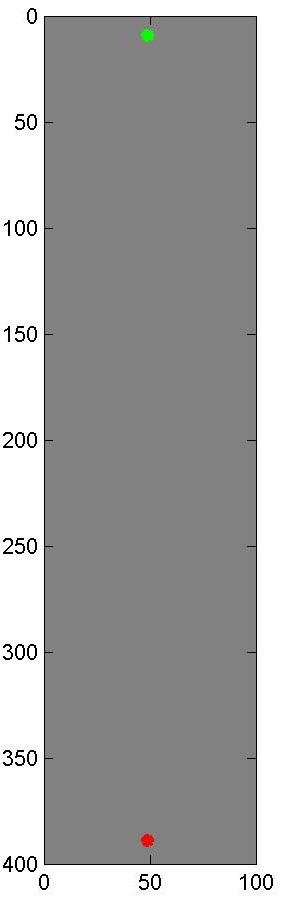
\includegraphics[width=0.75\textwidth]{figures/initialModel}
\end{center}
\caption{Initial layered Earth model.}
\end{figure}



\subsubsection{Seismic borehole tomography}
 A simple borehole tomography experiment was chosen to demonstrate the adaptive design method. The experiment measures the travel times between sources $n_s$ and receivers $n_r$. Travel times are given by integrating the slowness  $m(t,\vx)$ , or inverse acoustic velocity of the media,  along a ray path $\Gamma$,
\begin{equation*}\label{eq:tomo}
\bfd_{j,k}(t) =  \int\limits_{\Gamma_{j,k}} m(t,\vx)\, d\ell.
\end{equation*}
 Assuming the data are noisy and measured at times $(t_0,...t_n)$ the tomography problem is given by 
 \begin{equation*}
 \CF m(t_{k},\vx) + \epsilon_{k}  = \bfd(t_{k}).\\
\end{equation*}

Equation \eqref{eq:tomo} is discretized on a standard staggered 2D grid using a finite volume scheme placing $s$ and $\bfd$ at the cell centers, see figure \ref{fig:stag} below. 

The discrete tomography experiment in matrix form is then,
\begin{equation}
 	\bfF{\bfm_k} = \bfd_k, \text{ for } k=1,\ldots,n.
\end{equation}

The initial survey setup is pictured in figure \ref{fig:surveyDesign}, and includes 4 boreholes with 12 sources in the east borehole,  10 receivers in each center borehole,  20 receivers in the west borehole, and 20 surface receivers. The initial design was chose to overly cover all the area in the flow domain, with the goal of significantly reducing the number of data required. 
\begin{figure}[!h]
	\renewcommand{\arraystretch}{1.5}
	\begin{center}
		\iwidth=100mm
		\begin{tabular}{@{}|@{}c@{}|@{}c@{}|@{}} %{@{}|@{\ }p{3mm}@{}|@{\ }c@{\;}|@{\;}c@{\ }|}
			\hline		
			Experiment set-up 
			&
			Tomography rays 			
			\\
			\hline		
			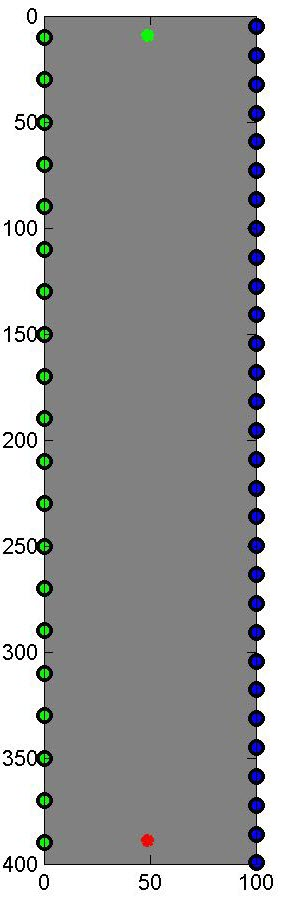
\includegraphics[width=.8\iwidth]{figures/initialExperimentNoRays}
			&
			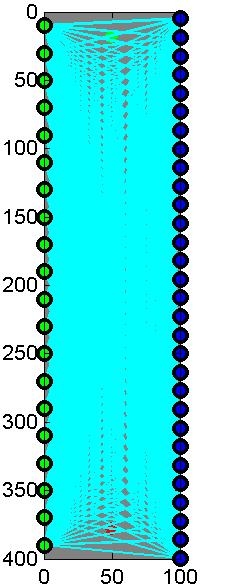
\includegraphics[width=.8\iwidth]{figures/initialExperiment}
			\\
			\hline
		\end{tabular}
	\end{center}
	\caption{Initial experiment setup. Sources are pictured in green on the left and receivers in blue on the surface, two 75m boreholes, and the right 100m borehole. The initial setup covers the entire flow domain with 12 sources and 60 receivers.}
	\label{fig:surveyDesign}
\end{figure}



\subsubsection{Tracer dynamics} 
 The subsurface dynamics are described by the  tracer advection equations as presented in \cite{Chen2006}, which characterize  the transport of a solute in a fully saturated porous media, 
\begin{subequations}
%\label{floweq}
\begin{eqnarray}
 \label{eq:flow}
&&\frac{\partial( c \rho)}{\partial t} + \div c \rho \vu  = 0,\\
\nonumber
 &&\text{ subject to } c\rho(0,\vx) = c_0\rho(\vx),
\end{eqnarray}
  with hydraulic conductivity $\bfK$, and tracer concentration $c$ in a fluid of density $\rho$. The fluid velocity field $\vu$ satisfies a simple source-sink ($q$) flow model
\begin{eqnarray}
\label{eq:flowp}
&&  \div  \vu =   q \\ % \mu^{-1}\bfK(\bfx) \grad p
\label{eq:flowu}
&& \vu =  \bfK(\vx)  \grad p \\
\label{eq:incond}
&&  p(0,\vx) = p_0(\vx),
\end{eqnarray}
\end{subequations}
 with either Dirichlet or Neumann boundary conditions on the pressure $p$.\\
 
With the goal being to image the motion of the tracer, $c(t,\vx)$, we assume that changes in $c$ amount to changes in geophysical properties. This implies that $m(c)$ exists, and that the motion of $m$ is governed by Equation \eqref{eq:flow}. From  now on we will refer only to $\bfm$. 

%
\begin{figure}[h!]
\begin{center}
\	\includegraphics[width=0.75\textwidth]{figures/flow}
\end{center}
\caption{Velocity field(arrows) and the initial tracer concentration used to generate data}
\end{figure}
To discetize the advection of the tracer, a particle in cell discretization was chosen such that equation \eqref{eq:flow} is then given by,
\begin{equation*}
\bfm _k= \bfT(\bfu)\bfm_{k-1}. 
\end{equation*}

The remainder of the flow equations were disretized on a staggered grid using the finite volume method, with the components of the velocity field located on the cell edges and the tracer concentration at the cell centers. 

The  fluid velocity field $\bfu$ was  computed by solving equations \eqref{eq:floweq} with hydraulic conductivities for $\bfK$ ranging from $3e-1 \text{to } 6e-06 kg/s^2m^2$, and was time invariant. 


\begin{figure}[!h]
\label{fig:cell}
\begin{center}
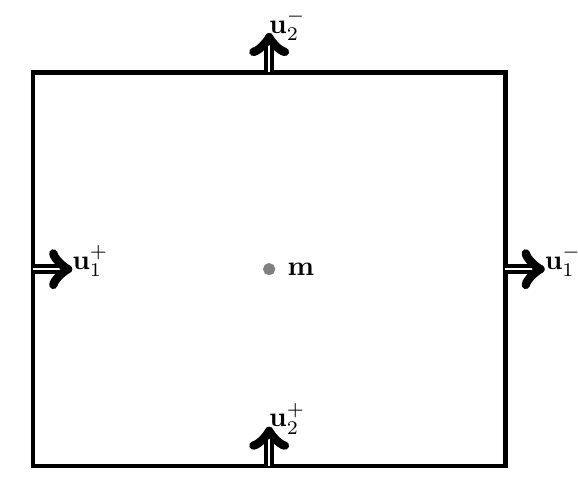
\begin{tikzpicture}[scale=1]
 	\draw[ultra thick]  (0,0) -- (6,0) -- (6,5) -- (0,5) -- cycle;
	\draw[black,ultra thick,double,->] (0,2.5) -- (0.5,2.5);
	\draw[black,ultra thick,double,->] (6,2.5) -- (6.5,2.5);
       \draw[black,ultra thick,double,->] (3,0) -- (3,0.5);
       \draw[black,ultra thick,double,->] (3,5) -- (3,5.5);
       
       %\draw[blue,ultra thick,double,->] (2,-2.5) -- (1,-2.7);
       %\draw[blue,ultra thick,double,->] (3.5,0) -- (3.5,1);
       %\draw[blue,ultra thick,double,->] (6,-2) -- (7,-2);
      \draw [gray,fill] (3,2.5) circle (2pt);
       \pgfputat{\pgfxy(3,2.5)}{\pgfbox[left,center]{\ \ $\bfm$}};
      \pgfputat{\pgfxy(0.5,2.6)}{\pgfbox[left,center]{$\bfu_{1}^{+}$}};
      \pgfputat{\pgfxy(6.5,2.6)}{\pgfbox[left,center]{$\bfu_{1}^{-}$}};
      
      \pgfputat{\pgfxy(3.0,0.6)}{\pgfbox[left,center]{$\bfu_{2}^{+}$}};
      \pgfputat{\pgfxy(3.0,5.6)}{\pgfbox[left,center]{$\bfu_{2}^{-}$}};
      

       \end{tikzpicture}
\caption{An example of a stagered grid cell with model parameters at the cell center and fluid velocity field on the edges. \label{fig:stag}}
\end{center}
\end{figure}
 
%\subsubsection{Comparing solution methods} % (fold)
%To compare solutions methods, an experiment was conducted where data were collected from all source receiver combinations allowed. Initial estimates of $\Sig_0$ and the best Tikhonov regularization parameter $\alpha_0$ were obtained by a standard cooling algorithm and Pareto curve. All three solution methods were considered for a small problem. The inverse prior covariance matrix was computed explicitly, and the full system was solve. The lanczos method was used by factoring the explicit prior covariance, and finally the krylov method was used such that nothing was formed or computed explicitly. 
%\todo[inline]{did this for one time step. works fine. krylov takes for ever. Had to go to super good 1e-9 accuarcy and high iterations to get a solution that matches the others. Weights very sensitive to how accurate this was solved}

\subsubsection{Regularization}
Next, the regularization functionals  for the  tracer estimation are discretized. For the  linear regularization  term $\hf\|\bfL \bfm\|^2_2 $, the operator $\bfL = \GRADh$ is a standard 2-point discretization of the gradient of a cell-centered variable, and has the effect of smoothing the solution.

A nice choice for a non-linear regularization operator for this problem is smoothed Total Variation~\cite{ahh}, since the tracer experiencing advective flow with no diffusion can have discontinuities. 
\begin{equation}
		\CRsat(s_0) = \beta \int  \phi(|\grad s_0|) \ d\vx.
\end{equation} 

Again, noting that $\bfm$ is discretized on a cell-centered grid, a standard discrete 
approximation for the smoothed total variation regularization is applied
\begin{equation*}
\label{eq:nonLinReg}
R^{m}(\bfm) = h^2 \bfe^{\top} \sqrt{ \bfA_{f}^{c} \left( (\GRADh\ \bfm) \odot (\GRADh\ \bfm) \right)  + \epsilon},
\end{equation*}
where $\GRADh$ is a standard 2-point discretization of the gradient of a cell-centered variable, which maps from cell-centers to faces, as described in~\cite{ha,ahh}.
$\bfA_{f}^{c}$ is an averaging matrix from cell-faces to cell-centers.
Note that we somewhat abuse the notation, and that the square root of a vector is the point-wise square root.

\subsection{Results}
To generate data, an initial tracer concentration was marched along in time, for time steps of 90 days, with Gaussian noise added. In total 6 experiments were conducted every 90 days. 

The initial design for time point 1 did not include the dynamics. This is basically the static case, or when there has been no data collected. In algorithm \ref{Alogrithm} this amounts to setting $\bfF_k = 0$ and the transport matrix $\bfT = \bfI$. 
Figure \ref{t1} shows the  variance, equation \eqref{ABk}, as a function of the number of non zero weights (nnz).  
\begin{figure}[!h]
	\renewcommand{\arraystretch}{1.5}
	\begin{center}
		\iwidth=100mm
		\begin{tabular}{{|@{}c@{}|@{}c@{}|}} %{@{}|@{\ }p{3mm}@{}|@{\ }c@{\;}|@{\;}c@{\ }|}
			\hline		
			Sparsity
			&
			Weights			
			\\
			\hline		
			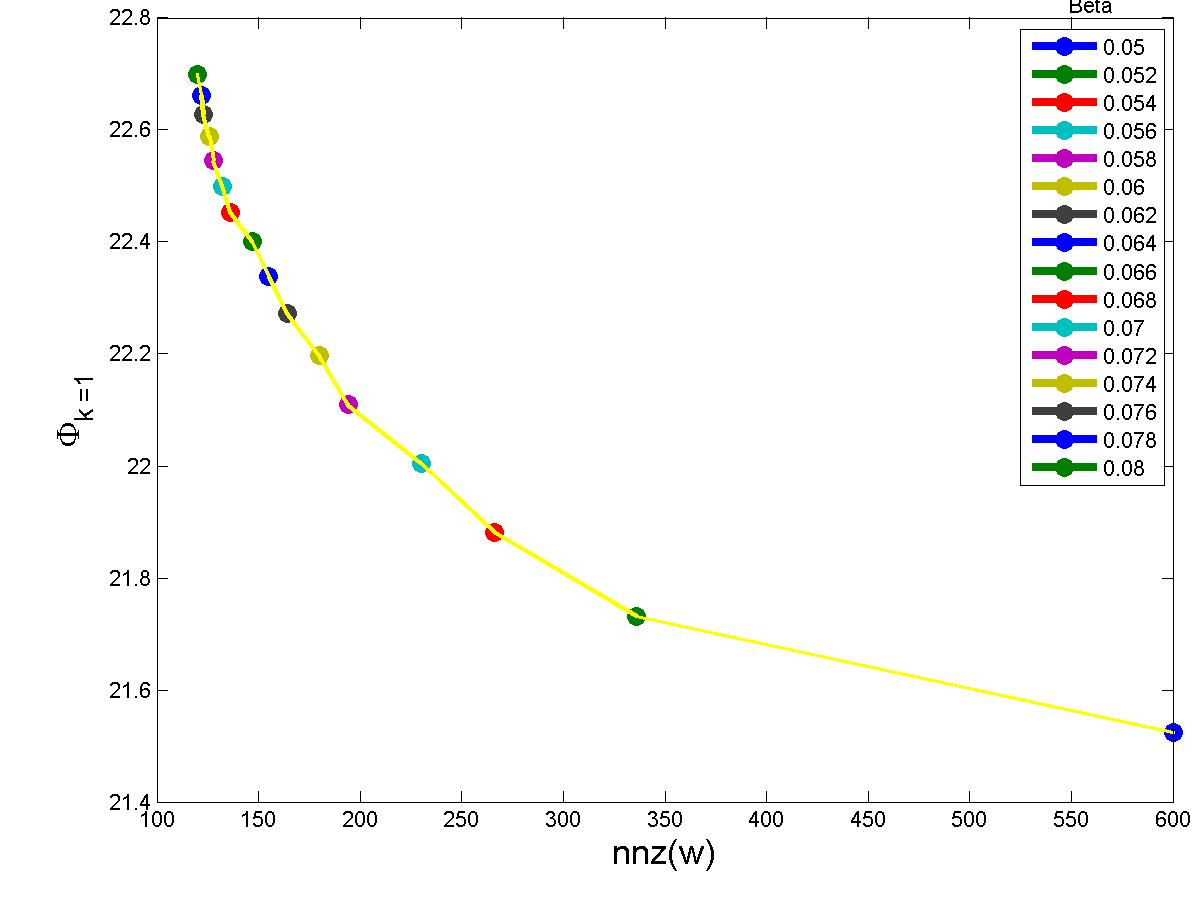
\includegraphics[width=.8\iwidth]{figures/exp1paretoWeights}
			&
			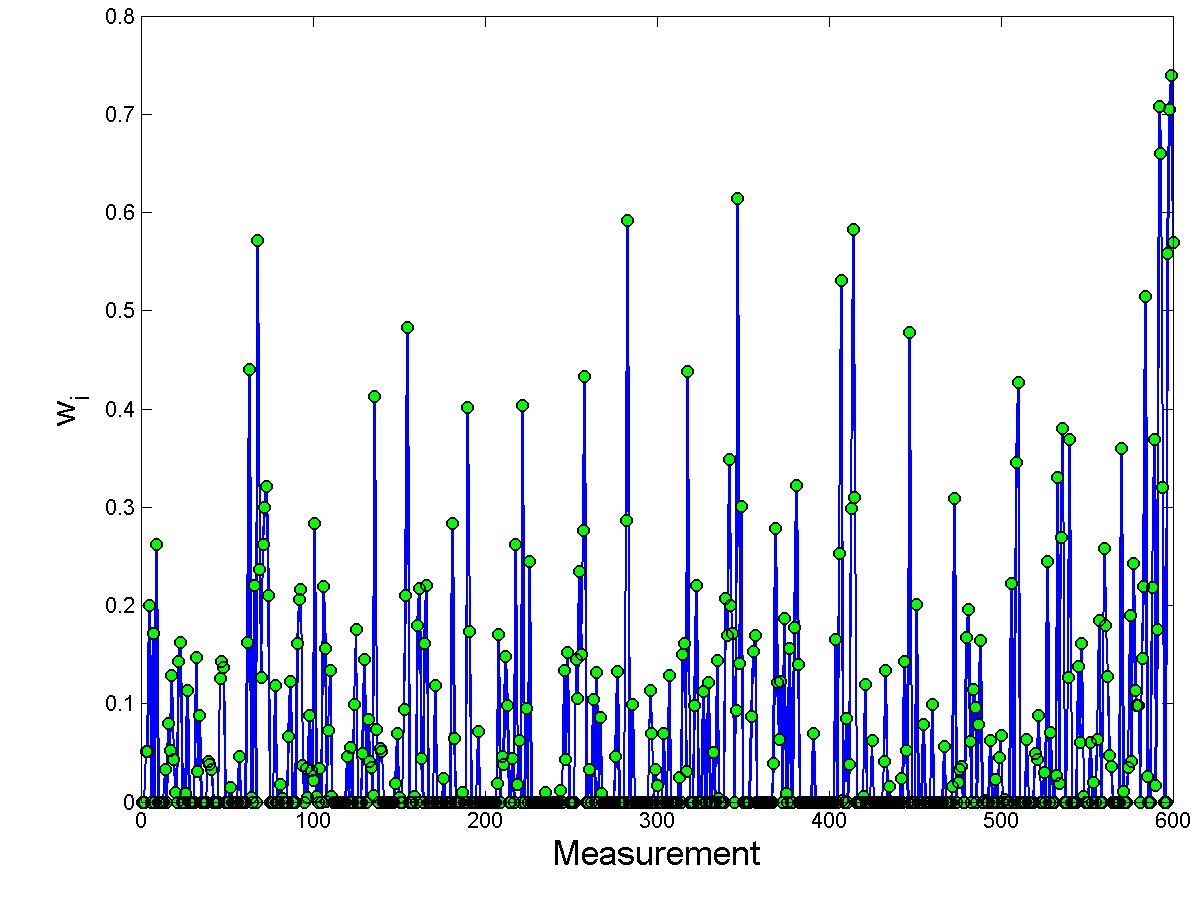
\includegraphics[width=.8\iwidth]{figures/exp1Weights}
			\\
			\hline
		\end{tabular}
	\end{center}
	\caption{Plot of variance $\phi_1(\bfw)$ versus $\bfw$, and the weights for $\beta = 1$ }
	\label{fig:weights1}
\end{figure}
We chose $\beta =1$ which corresponds with about 399 of the 720 data being used. The new design and the recovered model of the tracer are presented below.
\begin{figure}[h!]
\begin{center}
\	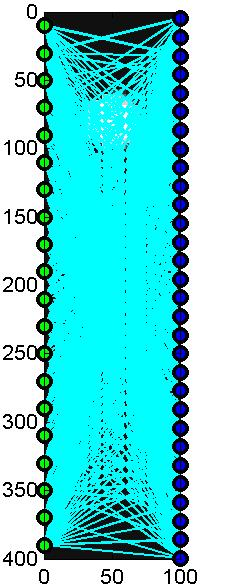
\includegraphics[width=0.75\textwidth]{figures/resultsExp-1-designs}
\end{center}
\caption{An image of the optimal design data, or rays plotted over the full set of rays The number of data required was decreased from 720 to 399}
\end{figure}
\begin{figure}[!h]
	\renewcommand{\arraystretch}{1.5}
	\begin{center}
		\iwidth=100mm
		\begin{tabular}{{|@{}c@{}|@{}c@{}|}} %{@{}|@{\ }p{3mm}@{}|@{\ }c@{\;}|@{\;}c@{\ }|}
			\hline		
			true model k = 0
			&
			recovered model (TV) 399 data	
			\\
			\hline		
			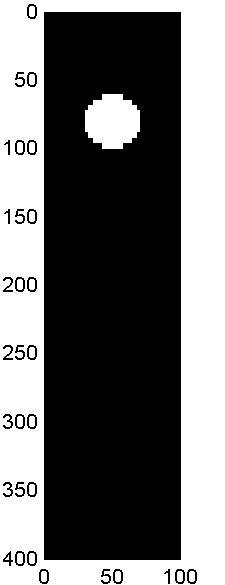
\includegraphics[width=.8\iwidth]{figures/resultsExp-1-mtrue}
			&
			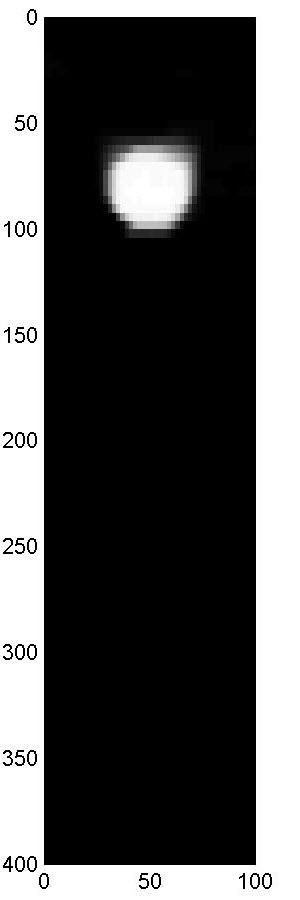
\includegraphics[width=.8\iwidth]{figures/resultsExp-1-mkTV}
			\\
			\hline
			recovered model 720 data 
			&
			recovered model 399 data	
			\\
			\hline		
			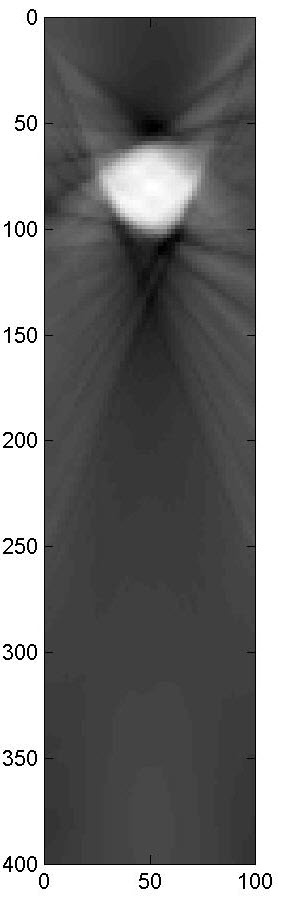
\includegraphics[width=.8\iwidth]{figures/resultsExp-1-mAlldata}
			&
			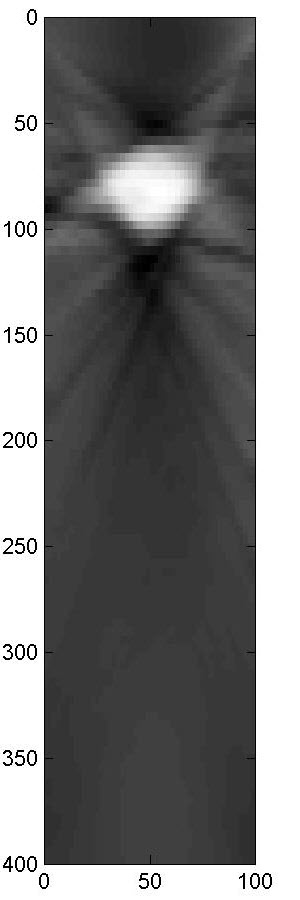
\includegraphics[width=.8\iwidth]{figures/resultsExp-1-mk}
			\\
			\hline
		\end{tabular}
	\end{center}
	\caption{Static optimal design, $k=0$. The 4 panels show the true tracer and subsurface, the image recovered using 399 data points and total variation for the regularization, and recoveries using all data and the optimal data for the linear gradient regularization}
	\label{fig:results1}
\end{figure}

\begin{figure}[!h]
	\renewcommand{\arraystretch}{1.5}
	\begin{center}
		\iwidth=100mm
		\begin{tabular}{{|@{}c@{}|@{}c@{}|}} %{@{}|@{\ }p{3mm}@{}|@{\ }c@{\;}|@{\;}c@{\ }|}
			\hline		
			Sparsity
			&
			Weights			
			\\
			\hline		
			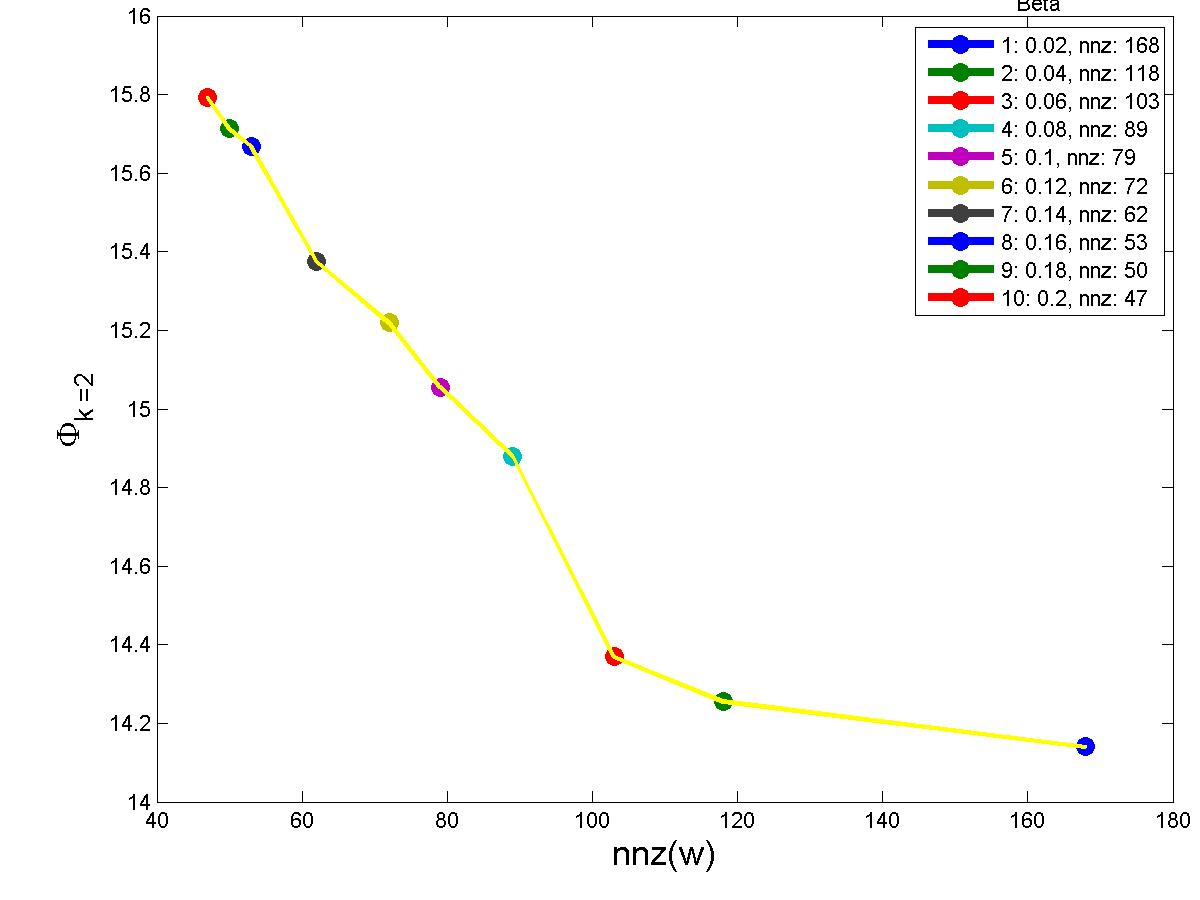
\includegraphics[width=.8\iwidth]{figures/exp2paretoWeights}
			&
			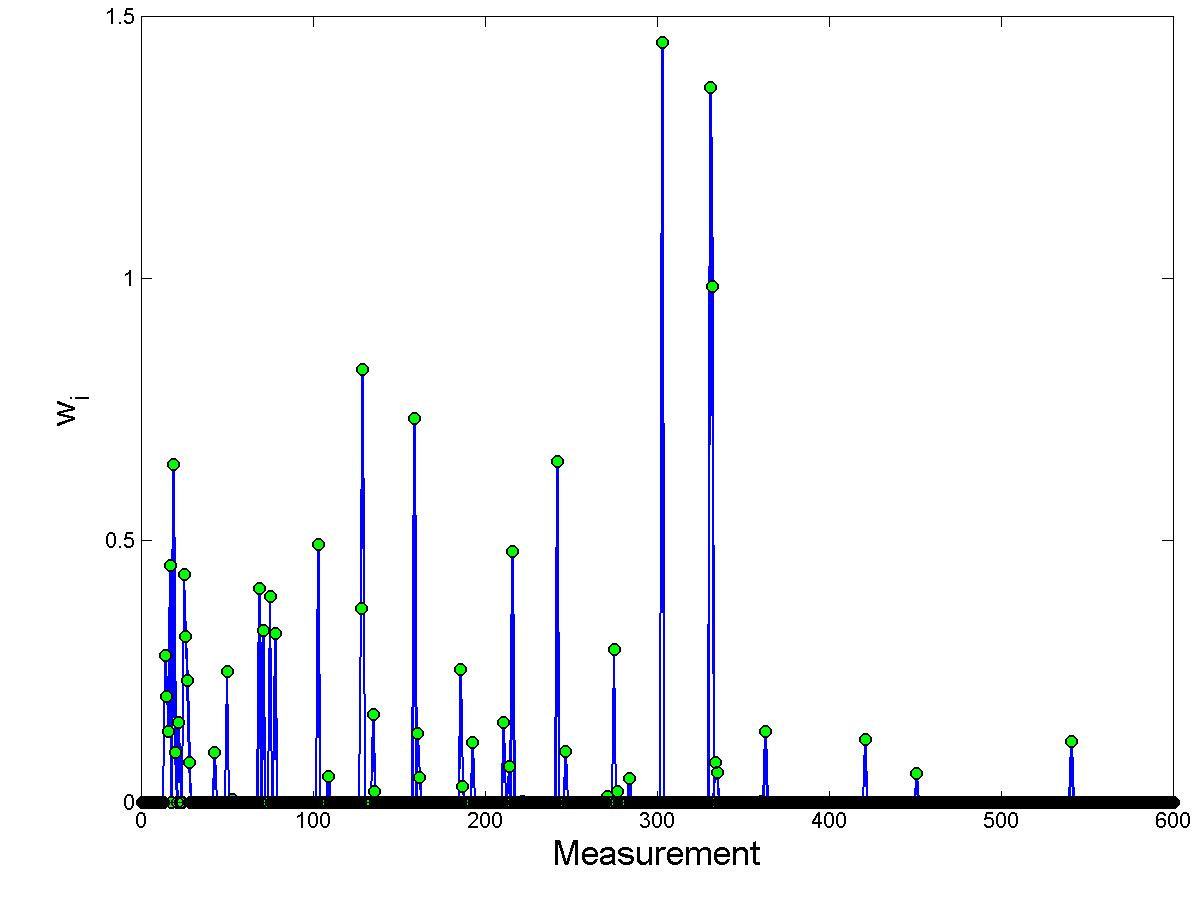
\includegraphics[width=.8\iwidth]{figures/exp2Weights}
			\\
			\hline
		\end{tabular}
	\end{center}
	\caption{Experiment k = 1. Plot of variance $\phi_1(\bfw)$ versus $\bfw$, and the weights for $\beta = 1$ }
	\label{fig:weights1}
\end{figure}

\begin{figure}[!h]
	\renewcommand{\arraystretch}{1.5}
	\begin{center}
		\iwidth=100mm
		\begin{tabular}{{|@{}c@{}|@{}c@{}|}} %{@{}|@{\ }p{3mm}@{}|@{\ }c@{\;}|@{\;}c@{\ }|}
			\hline		
			true model k = 1
			&
			recovered model (TV) 396 data	
			\\
			\hline		
			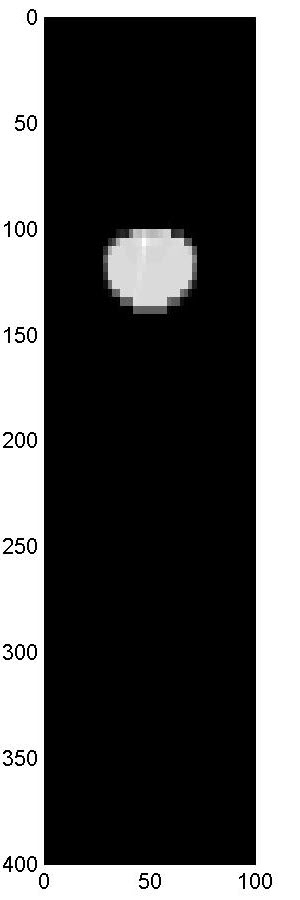
\includegraphics[width=.8\iwidth]{figures/resultsExp-2-mtrue}
			&
			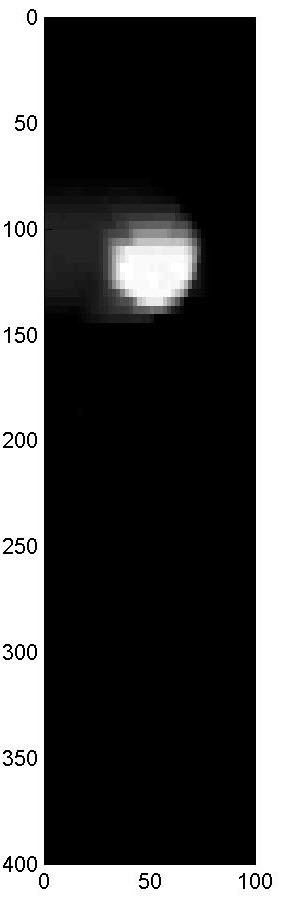
\includegraphics[width=.8\iwidth]{figures/resultsExp-2-mkTV}
			\\
			\hline
			recovered model 720 data 
			&
			recovered model 396 data	
			\\
			\hline		
			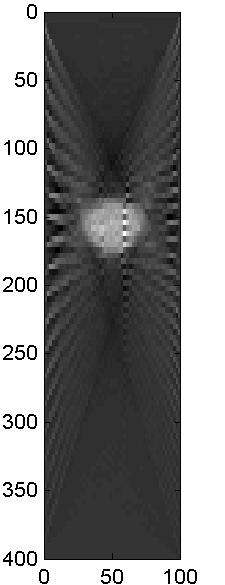
\includegraphics[width=.8\iwidth]{figures/resultsExp-2-mAlldata}
			&
			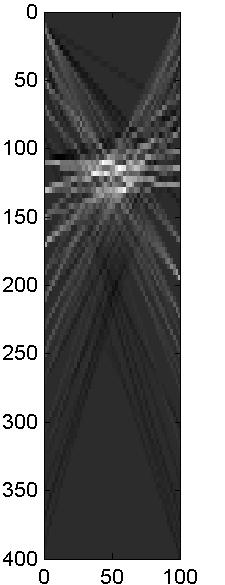
\includegraphics[width=.8\iwidth]{figures/resultsExp-2-mk}
			\\
			\hline
		\end{tabular}
	\end{center}
	\caption{Adaptive optimal design, $k=1$. The 4 panels show the true tracer in the subsurface after 90 days. The images were recovered using 396 data points for both the total variation and gradient regularization}
	\label{fig:results1}
\end{figure}













\section{Numerical example 2: Helmhotz maybe} 
This depends on how far ahead in time we design...The all at once approach assumes the velocity field is accurate(ish)...could still solve the all at once problem for updated velocity field too. 



\section{Concluding Remarks}






\bibliographystyle{plain}
\bibliography{../../../../Bibliographys/ProposalBib}



\end{document}